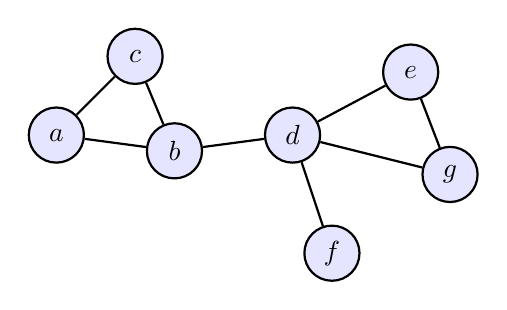
\begin{tikzpicture}[
  vnode/.style={circle, draw, minimum size=7mm, inner sep=0pt, fill=blue!10},
  thick
]
  \node[vnode] (a) at (0, 1) {$a$};
  \node[vnode] (c) at (1, 2) {$c$};
  \node[vnode] (b) at (1.5, 0.8) {$b$};
  \node[vnode] (d) at (3, 1) {$d$};
  \node[vnode] (e) at (4.5, 1.8) {$e$};
  \node[vnode] (g) at (5, 0.5) {$g$};
  \node[vnode] (f) at (3.5, -0.5) {$f$};
  
  \draw (a) -- (b);
  \draw (a) -- (c);
  \draw (c) -- (b);
  \draw (b) -- (d);
  \draw (d) -- (e);
  \draw (e) -- (g);
  \draw (g) -- (d);
  \draw (d) -- (f);
\end{tikzpicture}
\par\medskip
\textit{Obrázek 1.3: Sekvence $a, b, d, e, g, d, f$ je sled, ale ne cesta (opakuje se vrchol $d$). Sekvence $a, b, d, f$ je cesta.}